\documentclass[a4paper]{article}

\usepackage{fullpage} % Package to use full page
\usepackage{parskip} % Package to tweak paragraph skipping
\usepackage{tikz} % Package for drawing
\usepackage{amsmath}
\usepackage{hyperref}
\usepackage{amssymb}

\usepackage{enumitem}

\usepackage{tkz-graph}
\usepackage{float}

\title{11 An Introduction to Graph Theory}
\author{Ling Tan}
\date{2018-10-11}

\begin{document}

\maketitle

\section*{11.1 Definitions and Examples}
\textcolor{blue}{Definition 11.1}: Let $V$ be a finite nonempty set, and let $E\subseteq V\times V$. The pair $(V,E)$ is then called a directed graph (on $V$) or digraph (on $V$), where $V$ is the set of vertices, or nodes, and $E$ is its set of (directed) edges or arcs. We write $G=(V,E)$ to denote such a graph.

\textcolor{blue}{Definition 11.2?}: Let $x,y$ be (not necessarily distinct) vertices in an undirected graph $G=(V,E)$. An $x-y$ walk in $G$ is a (loop-free) finite alternating sequence
$$
x=x_0,e_1,x_1,e_2,x_2,e_3,\ldots,e_{n-1},x_{n-1},e_n,x_n=y
$$

\textcolor{blue}{Definition}: $u=u_0, e_1, u_1, e_2, u_2, \ldots, e_{n-1},u_{n-1}$

trail: no repetition of edges?
path: is trail, no repetition of vertices
circuit: no repetition of edges?
cycle: is path starts and end with the same vertex.

\textcolor{blue}{Definition}: Graph $G=(V,E)$ is called connected if there is a path between any two distinct vertices of $G$. A graph is not connected is called disconnected.

\textcolor{blue}{Definition}: 
\textcolor{blue}{Definition}: Let $V$ be a set of $n$ vertices. The complete graph on $V$ denoted $K_n$, is a loop-free undirected graph where all $a,b\in V, a\neq b$, there is edge $\{a,b\}$.


\section*{11.2 Subgraphs, Complements, and Graph Isomorphism}
\textcolor{blue}{Definition}: Let $G$ be a loop-free (undirecte) graph on $n$ vertices. The complement of $G$, denoted $\bar G$, is the subgraph of $K_n$ consisting of the $n$ vertices in $G$ and all edges that are not in $G$. Any complement graph of complete graph is null graph.


\textcolor{blue}{Definition}: Let $G_1=(V_1,E_1)$ and $G_2=(V_2,E_2)$ be two undirected graphs. A function $f:V_1\rightarrow V_2$ is called a graph isomorphism

\begin{center}
    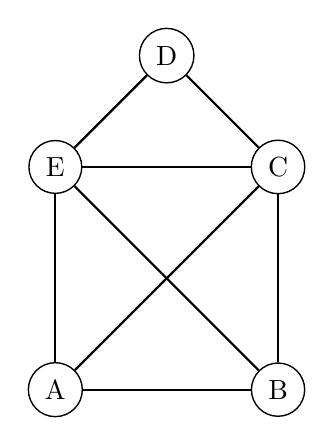
\begin{tikzpicture}
        \GraphInit[vstyle=Normal]
        \SetGraphUnit{2}
        \begin{scope}[rotate=-135]
            \Vertices{circle}{A,B,C,E}
        \end{scope}
        \NOEA[unit=1.414](E){D}
        \Edges(A,B,E,D,C,E,A,C,B)
    \end{tikzpicture}
\end{center}

\section*{11.3 Vertex Degree: Euler Trails and Circuits}
\section*{11.4 Planar Graphs}
\section*{11.5 Hamilton Paths and Cycles}
\section*{11.6 Graph Coloring and Chromatic Polynomials}
\section*{11.7 Summary and Historical Review}

\end{document}